\chapter{Foobaz: Feedback on Variable Names at Scale}\label{chapter:foobaz}

Current traditional feedback methods for solutions to programming assignments include hand-grading substance and style. Unfortunately, those methods are labor intensive, potentially inconsistent across graders, and do not scale to the sizes associated with Massive Open Online Courses (MOOCs). The scaling difficulty is particularly important when considering that  some residential course enrollments at prominent universities, like UC Berkeley's CS61A, are rising above the thousand-student mark \cite{biggestClass}. Some Computer Science teachers, such as MIT's John Guttag and Ana Bell, are simultaneously teaching hundreds of students in residential programming courses and thousands of online students in MOOC versions.

Variable naming is a specific, important aspect of writing readable, maintainable code, and many teachers want to give feedback on it. The quality of a name is most easily judged when its role within the surrounding code is known. However, at scale, teachers cannot read every solution. Programming education at scale opens up new challenges for processing and presenting thousands of solutions so that teachers can more easily view them. Teachers also cannot write comments on each solution. This difficulty motivates the creation of tools that help teachers give customized feedback to subsets of students for whom that feedback is relevant.

This chapter introduce Foobaz, a user interface for giving tailored feedback on student variable names at scale. Foobaz enables teachers to explore and comment on the quality of student-chosen variable names, given the role the variables play in student solutions (see Figure \ref{fig:figure2}). A variable's role is a function of the sequence of values that the variable contains during program execution. The variety of student-chosen variable names for each role makes evaluating every one prohibitive. Using Foobaz, the teacher can label a small subset of good and bad names for each role. 

Foobaz then uses these labeled variable names to create pedagogically valuable active learning exercises in the format of multiple choice quizzes. These quizzes are a form of feedback for many more students than just those whose variable names receive a teacher label. The quizzes also allow students to see examples of good and bad alternatives, rather than just receive a label on one of their own names. 

Foobaz personalizes teacher quizzes for each student, so that students can consider good and bad names for variables that exist in their own solutions. Personalized quizzes render the original student solution with a specific variable replaced by an arbitrary symbol. The quiz presents the student with several variable names as candidate replacements for the symbol, one of which may be the student's original choice. The student selects appropriate labels for the variable names before checking their labels against teacher labels and comments.

In two user studies, the capabilities and workflow enabled by this novel interface are demonstrated. The first study shows that the interface helped teachers give personalized variable name feedback on thousands of student solutions from an introductory programming MOOC on edX. In the second study, students composed solutions to the same programming exercises and received personalized quizzes generated with Foobaz by teachers in the first study.

\todo{remove we from the rest of this chapter}

\section{User Interface}

Consider an introductory programming MOOC where thousands of students submit correct solutions to a programming problem. Imagine that many of these solutions include a variable that takes on the same sequence of values, like a running sum of the elements in an input argument. While most students decide to name this variable \texttt{result}, others decide to give it obscure or less descriptive names like \texttt{p}, \texttt{val1}.

The quality of a variable's name is most easily judged when the teacher understands its algorithmic role and relationship to other variable names within the surrounding code. At scale, this can be difficult and frustrating, because while variable roles can be repetitive across many solutions, e.g., a particular running sum, their names can be unpredictable (\texttt{result}, \texttt{val1}, \texttt{s}). Instead of browsing student variable names in a linear fashion, it would be better if the teacher could provide feedback on the basis of variable roles.

In Foobaz, teachers can browse \emph{stacks} of student solutions represented by platonic solutions. A stack is a set of solutions whose code is identical after standardizing formatting, normalizing variable names, removing comments, and ignoring the exact order of statements. Within a stack, the teacher can browse the different sets of variable names that students chose, label some of them as, e.g., ``too short'' or ``misleading,'' and add comments. 

Teacher labels and comments are used to provide students with tailored feedback in the form of personalized quizzes on variable names. By providing feedback on only a few variable names, personalized quizzes are generated that are potentially relevant to thousands of students. Foobaz is distinct from powergrading systems: instead of grading as many names as possible, the system produces personalized quizzes that have excellent examples of good and bad variable names students would not otherwise get to see and learn from.

\subsection{Producing Stacks and Common Variables}
The OverCode analysis pipeline executes each student solution on a test case and tracks the sequences of values that variables take on. Common variables are identified as those that behave the same way, i.e., take on the same sequence of values, across multiple solutions. After executing every solution, the OverCode pipeline groups solutions into stacks of similar solutions. Each stack is represented by a single platonic solution. In the Foobaz teacher view, the teacher browses the platonic solutions and annotates the quality of variable names for common variables. 

The stacking performed by the system directly reduces the number of implementations that a teacher needs to analyze in order to provide feedback to the majority of the class. Furthermore, Foobaz is sensitive to \emph{variable roles}, meaning that variables that behave the same across different stacks are linked together as a single common variable. The result is that feedback provided for a variable in one stack is propagated to variables that play out the same behavior in \emph{other} stacks.

\subsection{Rating Variable Names}

The Foobaz interface lets the teacher rate variable names in the context of their role in the program. Figure \ref{fig:figure2} shows the teacher view while they perform this task. 

The teacher is presented with a scrollable list of stacks. Each stack is represented as a platonic solution followed by a table of alternative variable names. Since some of the tables are taller than the screen, the platonic solution is pinned to the screen in such a way that it remains visible until the next stack is scrolled into view.

Each column of the table represents the common variables occurring in the stack, where each common variable's most popular name serves as the column header. Each row of the table represents a unique set of variable names used in a solution (e.g., \texttt{secretWord}, \texttt{lettersGuessed}, \texttt{guessedWord}, \texttt{char}). We show \emph{sets} of variable name choices, rather than independent columns of variable names, because we found in early pilot testing that variable names can at times make more sense when seen as a group, rather than as individual naming decisions. This helps give teachers the context and confidence to assign quality judgments.

As the teacher brushes over the names of a common variable in the table, its occurrences in the platonic solution are highlighted, so they can develop an understanding of the variable's role in the solution. The teacher can then go down the list of student-chosen names, rating as many of them as they desire using three different labels: ``misleading or vague,'' ``too short,'' or ``fine.'' These labels were based on early pilot testing with beginner programmers but future iterations of Foobaz may support teacher-added labels. Next to each name, they can also see how frequently it was given to that common variable across all solutions in the dataset, and can sort the entire table by this frequency. In order to draw teachers' attention to student-chosen variable names, variables with names that match one of given parameter names provided with the homework prompt are greyed out. The long tail of infrequently used names can be a place where both the best and worst examples of names can be found.

It is important to note that each common variable is likely to occur in multiple stacks. When the teacher selects a particular name, or set of names, for a common variable, occurrences in other stacks are highlighted as well. When they assign a label to a name, the label is propagated to all uses of the name for that common variable, across all the stacks. This has the effect of ``filling down'' the teacher annotations. As teachers scroll down, they see that much of their feedback has been propagated for them, letting them focus on the remaining best and worst examples they might find. 

A progress bar at the top of the page indicates the coverage of their feedback across all variable names. Since teachers were motivated by the progress bar to maximize their coverage, we provided a button which would select and scroll into view the next most popular, yet unlabeled name for a common variable. Also included to maximize efficiency, the interface supports navigation through the variable names in the table using arrow keys. Teachers can also press hotkeys to rate variables instead of clicking on one of the three quality judgments, e.g., press \texttt{2} to rate a variable name as ``too short.''

\begin{figure}
\centering
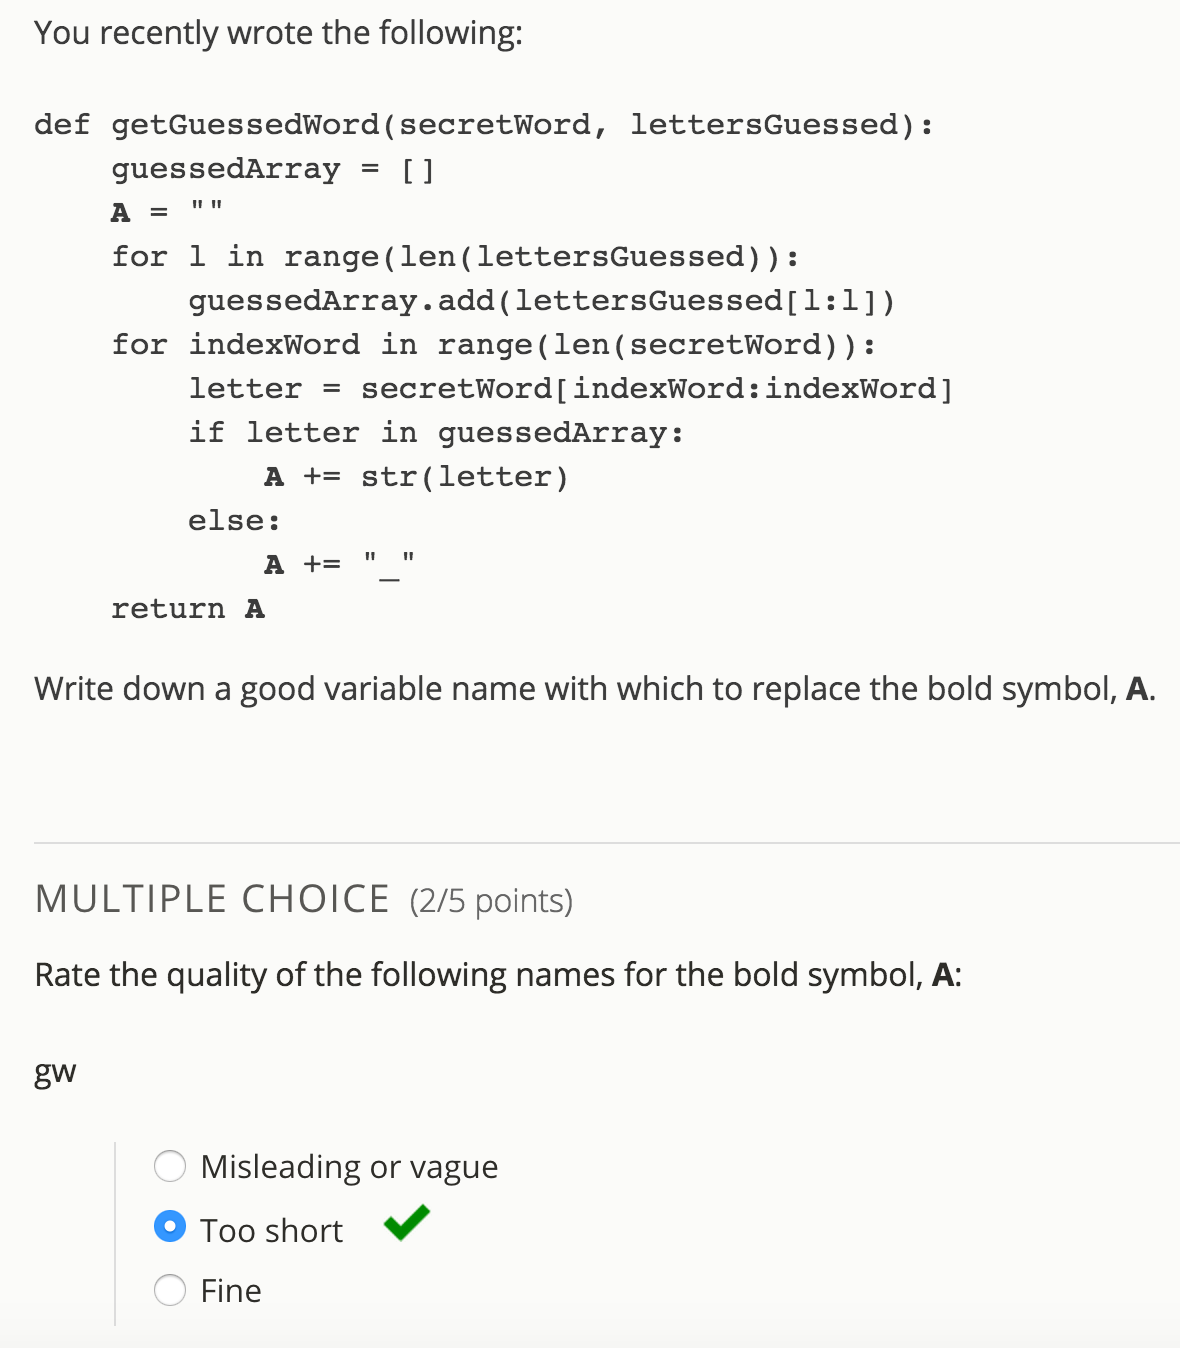
\includegraphics[width=0.95\columnwidth]{Body/figures/foobaz/feedbackQuizExample.png}
\caption{A personalized quiz as seen by the student, delivered by edX infrastructure. Students are shown their own code, with a variable name replaced by an arbitrary symbol, followed by variable names for the student to consider and label using the same labels that were available to the teacher. After the student has submitted their own judgments, the teacher labels are revealed, along with their explanatory comments.}~\label{fig:figure4}
\end{figure}

\begin{figure}
\begin{minipage}{1\columnwidth}
\centering
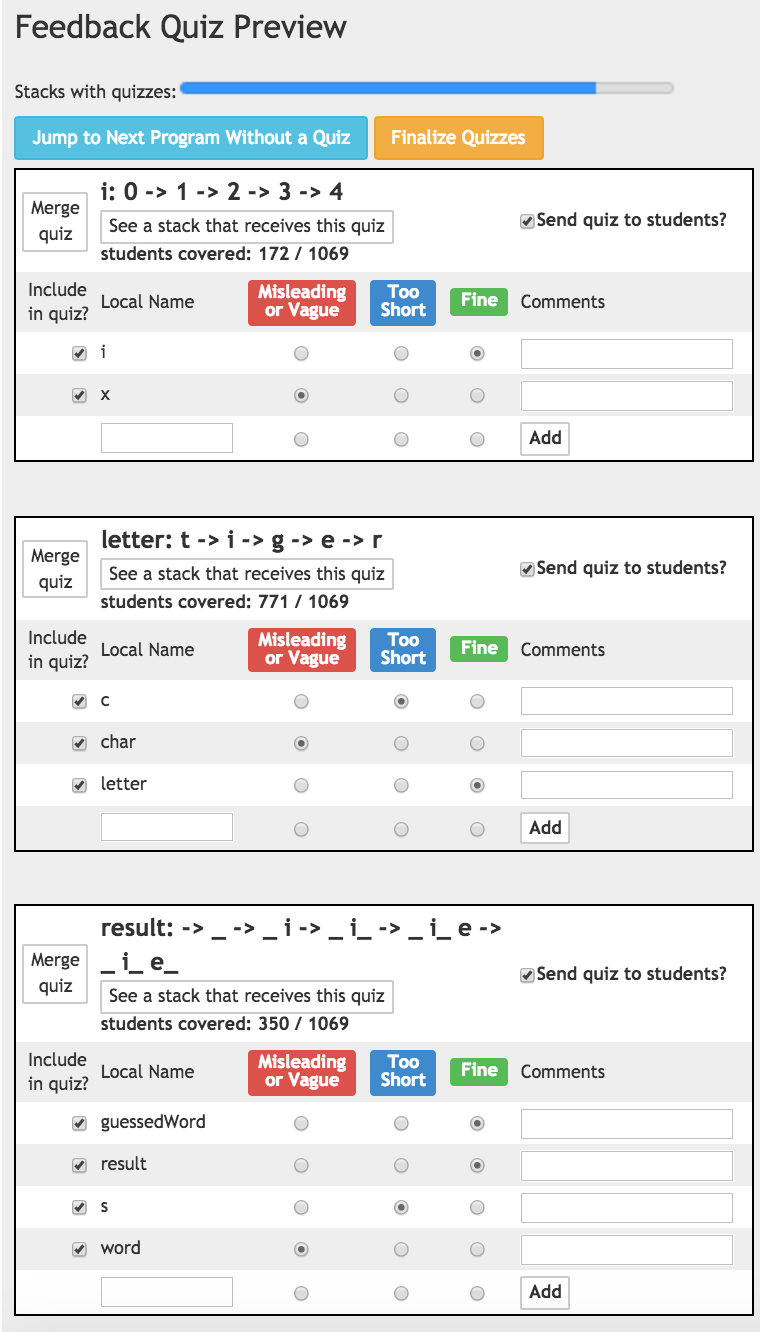
\includegraphics[width=0.85\columnwidth]{Body/figures/foobaz/quizPreviewHangman.png}
\caption{The quiz preview pane of the Foobaz teacher interface. Variable behavior was logged by running all solutions on a common test case. This particular teacher created quizzes for the common variable \texttt{i} that iterates through indices of a list, the common variable \texttt{letter}, which iterates through the characters in an input string, and the common variable \texttt{result}, which accumulates one of the acceptable return values, `\texttt{\_i\_e\_}.'}~\label{fig:figure3}
\end{minipage}

\bigskip
\begin{minipage}{1\columnwidth}
\centering
\begin{tabular} {|l|l|r|}
\hline
\tabhead{Problem Description} & \tabhead{Source} & \tabhead{Solutions} \\ \hline \hline
\codevar{iterPower} & 6.00x (edX) & 3875 \\ \hline
\codevar{hangman} & 6.00x (edX) & 1118 \\ \hline
\codevar{computeDerivative} & 6.00x (edX) & 1433 \\ \hline
\codevar{dotProduct} & 6.0001 (residential) & 229 \\ \hline
\end{tabular}
\caption{Number of solutions in datasets.}
\label{solutioncounttable}
\end{minipage}

\bigskip
\begin{minipage}{1\columnwidth}
\centering
\begin{tabular}{|l|r|r|r|r|}
\hline
\tabhead{Problem} & \tabhead{Misleading} & \tabhead{Too short} & \tabhead{Good} & \tabhead{Total names} \\
& \tabhead{or Vague} & & & \\ \hline \hline
\codevar{iterPower} & 3 & 3 & 15 & 929 \\ \hline
\codevar{hangman} &7 & 4 & 10 & 763 \\ \hline
\codevar{compDeriv} & 6 & 5 & 10 & 670 \\ \hline
\codevar{dotProduct} & 11 & 3 & 17 & 180 \\ \hline
\end{tabular}
\caption{Subjects in Study 1, on average, labeled a small fraction of the total names, covering all three provided name categories.}~\label{tab:averageLabeling}
\end{minipage}

\end{figure}

\subsection{Making Quizzes}

Each quiz is an active learning exercise that asks the student to think about good and bad names for a common variable. Quizzes begin by showing a solution with that common variable's name replaced by an arbitrary symbol everywhere it occurs. In a personalized quiz, the solution is the student's own, as shown in Figure \ref{fig:figure4}. The quiz presents the student with several variable names as candidate replacements for the symbol, one of which may be the student's original choice. The student labels these names before checking their labels against the teacher's. If a student solution includes a particular common variable, then that student can receive a personalized version of the quiz about that variable.

As teachers rate variables by attaching labels to them, quizzes are created with these names as their good and bad examples. Using the Toggle Quiz Preview button, teachers can see a preview of the quizzes (Figure \ref{fig:figure3}) alongside the scrollable list of stacks and watch the quizzes grow as they rate more names. They can hide the quiz preview to reduce visual clutter while they explore all the stacks, common variables, and interesting alternative names.

If two different common variables perform the same conceptual role in student solutions but do not go through the exact same sequence of values, then the teacher can use the ``Merge'' button to combine the quizzes about each common variable into a single quiz. This quiz becomes relevant to students who have either common variable in their own solution and can be sent out to both groups.

Ultimately, the teachers' goal is to provide pedagogically valuable personalized quizzes to as many of the hundreds or thousands of students in the course as possible. Analogous to the progress bar for variable names, the quiz preview pane includes a progress bar for the number of stacks of solutions that will receive at least one quiz. Like the previously discussed button for selecting the next most popular unlabeled name, the quiz preview pane also includes a button for jumping to the next largest stack of student solutions that do not yet have any quizzes. If the teacher deems one of their automatically populated quizzes to be not pedagogically valuable, then they can uncheck the option to send that quiz back to students. To provide more illustrative examples that might not have been produced in student solutions, teachers can add their own custom good and bad variable name examples and write explanations in the comment field associated with each alternative name.

\section{Evaluation}

We evaluate the Foobaz teacher and student interfaces with two consecutive user studies, one for each population. In order to evaluate the scalability of Foobaz, the solutions seen by teachers were collected from MOOCs with thousands of students and a residential college class of several hundred students.

\subsection{Datasets}

We evaluated Foobaz on sets of correct solutions to four different programming problems, ranging in size from a couple hundred to several thousand solutions, collected from 6.00x, an introductory programming course in Python that was offered on edX in the fall of 2012, and 6.0001, a residential introductory programming course in Python offered at MIT in the fall of 2014 (see Figure \ref{solutioncounttable}). The four exercises, referred to here as \codevar{iterPower}, \codevar{hangman}, \codevar{dotProduct}, and \codevar{computeDerivative}, are representative of typical exercises that students solve in the early weeks of an introductory programming course. They have varying levels of complexity and ask students to perform loop computation over three fundamental Python data types, integers, strings, and lists.

\subsection{Teacher Study}

During the initial briefing, teachers were informed that they would be looking at solutions that had already passed an autograder and instructed to focus only on variable names, ignoring other aspects of code style, structure, and correctness. Teachers were invited to look over a page in a browser with all solutions concatenated in a random order into a flat list of boxed, syntax-highlighted code. We chose this design as our baseline to emulate existing methods of reviewing student functions. 

Using this baseline interface, teachers were asked first to rate as many good and bad variable names as possible, with an eye toward maximizing coverage of names (Task Part 1). Next, the teachers were shown an example of a quiz and were asked to compose their own by listing variable names and labeling them as good or bad with whatever short descriptors and explanatory comments they wished (Task Part 2). Participants were given 5 minutes for each task, and then asked to fill out a survey about their experience. (The answers to two of these surveys were lost so we only report survey results from 8 of the 10 participants.)

Participants learned about the Foobaz interface by watching a tutorial video. This training process took between 10 and 15 minutes depending on the dataset shown in the video. Participants were encouraged to hold their questions to the end, and answer them by interacting with the interface. 

Participants performed both Task Part 1 and 2 on a third dataset of solutions in the Foobaz teacher interface. Participants were asked to spend 5 minutes to perform each task, though some decided to spend more time. They filled out the same surveys about their experience again, followed by a final survey about which features of the Foobaz interface they found helpful. 

\subsubsection{Apparatus}

In all sessions, we used a laptop with a 15.4-inch 2880x1800 pixel Retina screen. All participants' interactions with the system were logged with timestamps using Meteor collections.

\subsubsection{Participants}

We recruited 10 participants (6 female) with ages between 20 and 29 ($\mu=23.1$, $\sigma=2.7$) through computer science-specific and campus-specific mailing lists and Facebook groups. All participants self-reported that they had been a grader, lab assistant, or teaching assistant for a Python course. 

\subsubsection{Results}

\textbf{Problems with Baseline}. When asked to comment on good and bad variable names based on the baseline interface, most teachers immediately began scrolling through solutions one by one, taking notes as they went, fully aware that they would only be able to skim a small, random fraction of the total number of solutions. The sheer volume of solutions was overwhelming to some. 

Results of the post-baseline survey reinforce critical usability issues with the status quo that Foobaz was designed to address. In these survey responses, teachers expressed an appreciation for the simplicity, readability, and searchability of the baseline interface but wished that the endless stream of often very similar solutions could be summarized or ``de-duped'' before they had to read through them. One teacher requested that variables be automatically identified, so that all references to a variable can be highlighted. This may have been a direct consequence of the fact that it was not possible to search for all the occurrences of the variable name \texttt{i} without the browser also highlighting all the \texttt{i}'s within the rest of the names and keywords, e.g., the \texttt{i} in ``if.'' Another teacher requested an automated count of common variable names. These teachers anticipated three critical features of the Foobaz interface: deduplication, variable name counts, and highlighting all occurrences of selected names.

Two teachers commented on the importance of understanding the role a variable takes on within the program. One teacher writes, ``Many times the variable names meant something but I still had to read the code to make sure that it meant what I thought it meant in the context of the code.'' The second teacher observed, ``Whether a variable name is good or bad depends a lot on its function within the code, and since each code block has a somewhat unique structure, I felt like I should be creating separate categories for good vs. bad variables names, e.g., `for the derivative result,' `for a counter in a loop through poly,' etc.'' This is exactly what the Foobaz interface is designed to support. 

\textbf{Power-law Distribution of Names}
The approximately power-law-type distribution of stacks of code from the thousands of edX solutions has already been reported in prior work, such as Figure 12 in \cite{overcode}. In Foobaz, the distribution of unique combinations of variable names and behaviors does not differ
significantly from a power-law distribution; the Kolmogorov-Smirnov test for a difference between the best-fitting power-law distribution and each dataset all gave p-values of at least $0.44$ (i.e., not significantly different), with the best-fitting exponent of the distribution between
$1.79$ and $2.13$. Within each stack, the names for any particular variable appear to follow the same distribution.

There is no ground truth for which variable names are ``bad,'' but we can report the counts of variables that the teachers chose to label and the counts of unique names for the top common variables in each problem. In the 3875 \codevar{iterPower} solutions, there were 179 different names given to a variable representing the base being exponentiated and 64 different names for a variable representing the exponent. In the 1393 \codevar{computeDerivative} solutions, there were 176 different names given for the variable containing the result and 39 different names for the most commonly used iterator variable. In the 1118 \codevar{hangman} solutions, there were 50 names given to the variable that iteratively takes on the characters of the secret word input argument and 99 names given to the variable containing the string most commonly returned by solutions as the answer. 

Figure \ref{tab:averageLabeling} shows the fraction of names that teachers labeled in Study 1, and the distribution of those names across various categories of quality. In spite of the unknown underlying distribution of good and bad variable names, the teachers find and label variables across all available categories in order to make quizzes.
 
\textbf{Efficiency of Foobaz}. The efficiency of using Foobaz to create feedback came up repeatedly in teachers' survey responses. Teachers appreciated the feeling of doing the task ``at scale.'' One teacher noted that it felt like, ``with each action, I was helping a large number of students'' without ``repeating or wasting effort too much.'' While using the button that highlights and scrolls the next most popular, untagged variable name into view, a teacher told the experimenter, ``I love this button!'' The arrow key-based navigation through tables of variable names was appreciated as well. At least one teacher commented that ``seeing variable names grouped by their role made the process much more efficient.'' 

The efficiency gains of the interface were hampered by, at times, a noticeably sluggish interface response time to some queries that scaled with the size of the dataset. This sluggishness can be cut down by reducing the many unnecessarily repeated calculations made in the current implementation.

\textbf{Quiz Composition}. In both interfaces, teachers appreciated the potential pedagogical value of making quizzes: ``I … liked that with the [quiz] I made, students can actually learn about good alternatives. ... [T]hey can change their variable names after putting extra thought into it.'' A teacher expressed appreciation that, using the Foobaz interface, they could generate quizzes based on actual submitted code as well as their own comments. 

\textbf{Coverage}. Immediately after using the baseline interface, teachers did not strongly agree or disagree with the statement ``I was able to give specific, personalized feedback to many students'' ($\mu =3$, $\sigma = 1.4$ on a 7-point Likert scale with 1: strong disagreement and 7: strong agreement). Teachers slightly disagreed with the statement ``I saw a large percentage of these students' variable names'' ($\mu=2.6$, $\sigma = 1.2$) and slightly agreed with the statement ``This interface helped me provide feedback to many students'' ($\mu=3.6$, $\sigma = 2.0$). After using the Foobaz interface, the mean level of agreement with these statements jumped to 5.5 ($\sigma = 1.7$), 6.3 ($\sigma = 0.46$), and 6.6 ($\sigma = 0.5$).

Figure \ref{fig:comboquizcoverage} shows that most solutions in the edX datasets received at least one or two quizzes. Solutions in  Figure \ref{fig:comboquizcoverage} have multiple common variables on which they could potentially be quizzed (3, 3, and 4 on average in subfigures (a), (b), and (c), respectively). One teacher used Foobaz to create quizzes for a much smaller dataset, collected from the residential class of only several hundred students. They achieved a similar percentage of coverage (87\% of student solutions received at least one quiz) in a similar amount of time, showing that the Foobaz workflow and output appears relatively invariant to the size of the dataset. Figure \ref{fig:variableCoverage} illustrates that, within minutes of their first interaction with the system, teachers can label a significant portion of student-chosen variable names in a dataset, though their progress trails off as they encounter the long tail of names for particular roles and transition to creating better quizzes.

Combined with Figure \ref{tab:averageLabeling}, Figure \ref{fig:comboquizcoverage} also shows that, by only labeling approximately 20 variable names in each of the edX datasets with thousands of student solutions, teachers cover at least 85\% of the class with personalized feedback quizzes. Even though Figure \ref{fig:variableCoverage} shows that the coverage of individual variable names with feedback is high, it matters less for Foobaz than in powergrading systems. What matters more is the coverage of students with quizzes that have excellent examples of good and bad variable names students would not otherwise get to see and learn from.

\begin{figure}
\begin{minipage}{1\columnwidth}
\centering
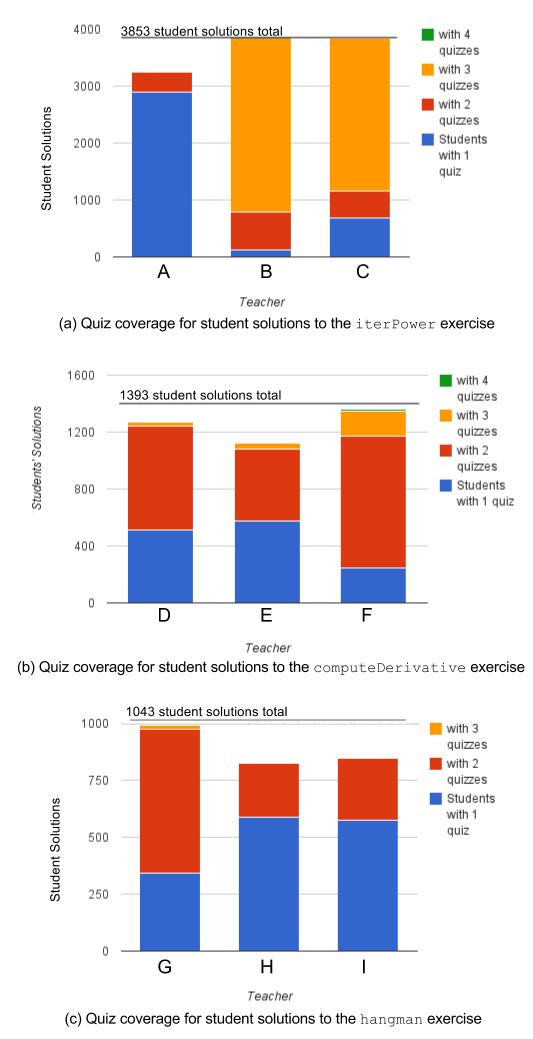
\includegraphics[width=1.0\columnwidth]{Body/figures/foobaz/ComboQuizCoverageFigure2.png}
\caption{Quiz coverage of student solutions across three datasets.}~\label{fig:comboquizcoverage}
%\end{figure}
\end{minipage}

\begin{minipage}{1\columnwidth}
%\begin{figure}
\centering
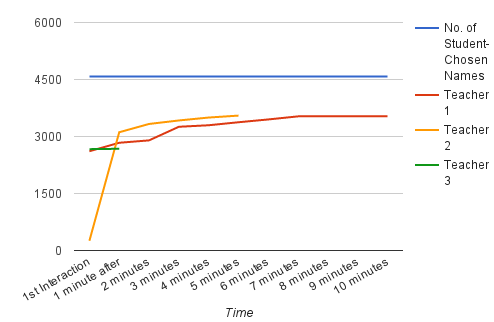
\includegraphics[width=0.9\columnwidth]{Body/figures/foobaz/variableCoverageNoTitle.png}
\caption{Variables in iterPower solutions labeled by each teacher.}~\label{fig:variableCoverage}
\end{minipage}
\end{figure}

\subsection{Student Study}

We ran a second study on the student side of the workflow in order to (1) find out if the teachers' efforts in the previous study produces quizzes that are relevant to these new students and (2) better understand student reactions to this novel form of feedback. In order to do this, we targeted beginner programming students and invited them into the lab to receive personalized quizzes generated by the teachers in our previous study.

Before the start of the study, quizzes composed by teachers using Foobaz in the first user study were rendered using the edX framework, ready to be personalized. Since pilot testing with beginner programming students indicated that six alternative variable names in a quiz is too many, teachers' quizzes were randomly subsampled to include a maximum of five alternative names for students to consider. 

Students came into the lab for one hour and composed solutions to one of the four exercises. After receiving each solution, the experimenter mentally executed the solution and compared the behavior of its variables to the variable behavior covered by the teachers' quizzes. If there was a match to one or more teachers' quizzes, one quiz was randomly selected. The experimenter made a copy of the student solution and replaced every instance of the variable to be quizzed on by an arbitrary symbol, e.g., a bold letter A. The experimenter then appended the quiz to the modified copy of the student solution and delivered it to the student as a personalized quiz. If there was no match to one or more teachers' quizzes, then the student received a generic quiz, about a variable name in a solution other than their own.

After the student completed their personalized quizzes, they took a survey about their experience. Students who were able to complete the coding exercise and quizzes with significant time left in their session repeated this process for a second programming problem.

\subsubsection{Apparatus}

In all sessions, we used laptops with 15.4-inch or 13.3-inch screens. All participants' interactions with the system were logged using the edX platform infrastructure.

\subsubsection{Participants}

We recruited 6 participants (4 female) who were either undergraduate or graduate students, through computer science-specific and campus-specific mailing lists, Facebook groups, and word of mouth advertising. Their ages were between 18 and 27 ($\mu=20.4$, $\sigma=3.2$). Four of the participants had taken one or two introductory programming courses on Coursera or at their high school or college campus. The remaining two participants had taken three or four classes that involved learning programming languages or computer science concepts, and had some experience with Python.

\subsubsection{Results}

Six students took a total of 12 quizzes, 11 of which were able to be personalized, even though their solutions were, in some cases, significantly different from the prior student solutions seen by teachers during quiz creation. Correspondingly, in the surveys that followed, students agreed with the statement ``This quiz felt relevant to me'' at an average level of 5.4 ($\sigma = 1.0$) on a 7-point scale. One student solution did not receive a personalized quiz because its variables behaved in ways that no teacher in the previous study considered. That student was able to understand the new solution and take the quiz, though it had little relation to their own solution.

Students were asked in the post-quiz surveys about what they learned from the exercise. One student replied, ``Possible variable names are pretty much synonyms, but the more detailed/specific ones are better.'' Another wrote, ``It's worthwhile to pick good variable names.'' Students' average level of agreement with the statement ``The quiz made me think about what makes variable names good or bad'' was 6.2 ($\sigma = 0.9$) on a 7-point scale. Mean levels of agreement with statements about the quizzes being confusing or tedious were 2.9 ($\sigma = 1.5$) and 3.4 ($\sigma = 1.2$), respectively, on a 7-point scale.

Some students observed that this was a very subjective quality of their code to be quizzed on, but all students were able to understand and complete the quizzes they were assigned. Some students disagreed with the instructor-provided ratings. When this occurred and the teacher left no explanation, students had at least one of three reactions: (1) They tried to imagine what the teacher was thinking. (2) They expressed displeasure at the lack of explanation. (3) They decided that they still disagreed with the teacher's judgment. Students did pick up on the teachers' preferred naming conventions through the quizzes. As evidence for this, two students correctly wondered aloud whether a different teacher made each of the quizzes they saw during their session. Given the subjectivity of the task, it may be necessary to grade only on participation, rather than absolute agreement with the teacher.

Students were not informed that quizzes were populated largely by fellow student variable names, but one student volunteered their appreciation for a ``wide spectrum'' of variable names to consider. However, randomly sampling teachers' quizzes down to 5 variable names created some student confusion when there were no positive naming examples in the resulting quiz. This is evidence that sampling should be constrained to include both good and bad examples and the user interface should provide some additional guidance to remind teachers that students highly value a balance of examples, each paired with an explanatory comment.

\section{Limitations}

The first study establishes the usability, learnability, and efficacy of
the main Foobaz interface for teachers. The second study is intended to
show that students can understand and use the personalized quizzes that
Foobaz produces. However, this evaluation of the student experience does not yet show pedagogical benefit. To measure learning benefits, we plan to deploy the tool in a
large Python programming course this fall.


\section{Conclusion}

We have designed and studied both the teacher and student sides of a novel interface and workflow for providing feedback on student variable names at scale. We hope it will serve as an example and a design pattern for future work on user interfaces for teaching programming to thousands of students at once.